%------------------------------------------------------------------------------
% Template file for the submission of papers to IUCr journals in LaTeX2e
% using the iucr document class
% Copyright 1999-2013 International Union of Crystallography
% Version 1.6 (28 March 2013)
%------------------------------------------------------------------------------

\documentclass[preprint]{iucr}              % DO NOT DELETE THIS LINE

  %----------------------------------------------------------------------------
  % Extra packages
  %----------------------------------------------------------------------------
  \usepackage{graphicx}         % For graphics
  \usepackage{mathtools}        % Math stuff
  \usepackage{bm}               % Bold in maths
  \usepackage{listings}         % Code snippets
  \usepackage{bold-extra}       % Bold mono space for code snippets
  \usepackage{url}              % For URLs
  \usepackage{xspace}           % Spacing in macros
  \usepackage{color}            % Colours
  \usepackage{textcomp}         % Required by listings when upquote=true
  \usepackage{multirow}         % Multirow spanning cells in tables
  \usepackage{siunitx}          % Proper formatting for units

     %-------------------------------------------------------------------------
     % Information about journal to which submitted
     %-------------------------------------------------------------------------
     \journalcode{J}              % Indicate the journal to which submitted
                                  %   A - Acta Crystallographica Section A
                                  %   B - Acta Crystallographica Section B
                                  %   C - Acta Crystallographica Section C
                                  %   D - Acta Crystallographica Section D
                                  %   E - Acta Crystallographica Section E
                                  %   F - Acta Crystallographica Section F
                                  %   J - Journal of Applied Crystallography
                                  %   M - IUCrJ
                                  %   S - Journal of Synchrotron Radiation

  %----------------------------------------------------------------------------
  % Bits of formatting used throughout document
  %----------------------------------------------------------------------------
  % program names
  \newcommand{\cctbx}{\emph{cctbx}\xspace}
  \newcommand{\rstbx}{\emph{rstbx}\xspace}
  \newcommand{\dxtbx}{\emph{dxtbx}\xspace}
  \newcommand{\lstbx}{\emph{lstbx}\xspace}
  \newcommand{\dials}{\emph{DIALS}\xspace}
  \newcommand{\dialsimport}{\emph{dials.import}\xspace}
  \newcommand{\dialsindex}{\emph{dials.index}\xspace}
  \newcommand{\dialsrefine}{\emph{dials.refine}\xspace}
  \newcommand{\dialsfindspots}{\emph{dials.find\_spots}\xspace}
  \newcommand{\xiatwo}{\emph{xia2}\xspace}
  \newcommand{\xds}{\emph{XDS}\xspace}
  \newcommand{\mosflm}{\emph{MOSFLM}\xspace}
  \newcommand{\madnes}{\emph{MADNES}\xspace}
  \newcommand{\fastmcd}{\emph{FAST-MCD}\xspace}
  \newcommand{\aimless}{\emph{AIMLESS}\xspace}
  % derivatives
  \newcommand{\pder}[2][]{\frac{\partial#1}{\partial#2}}
  \newcommand{\tder}[2][]{\frac{\mathrm{d}#1}{\mathrm{d}#2}}
  % use bold face for vectors
  \renewcommand{\vec}[1]{\mathbf{#1}}
  \newcommand{\uvec}[1]{\hat{\mathbf{#1}}}
  \newcommand{\mat}[1]{\mathbf{#1}}
  \newcommand{\rmat}[1]{\mat{R}_{#1}}

  % use to fix order in bibtex entries
  \newcommand{\mockalph}[1]{}

  % FIXMEs and visible comments
  \newcommand\fixme[1]{\textcolor{red}{#1}}

\begin{document}                  % DO NOT DELETE THIS LINE

     %-------------------------------------------------------------------------
     % The introductory (header) part of the paper
     %-------------------------------------------------------------------------

     % The title of the paper. Use \shorttitle to indicate an abbreviated title
     % for use in running heads (you will need to uncomment it).

\title{Detector metrology with DIALS}
%\shorttitle{Short Title}

     % Authors' names and addresses. Use \cauthor for the main (contact) author.
     % Use \author for all other authors. Use \aff for authors' affiliations.
     % Use lower-case letters in square brackets to link authors to their
     % affiliations; if there is only one affiliation address, remove the [a].

  \cauthor[a,b]{David G.}{Waterman}{david.waterman@stfc.ac.uk}{}
  \author[c]{Graeme}{Winter}
  \author[c]{Richard J.}{Gildea}
  \author[c,d]{James M.}{Parkhurst}
  \author[e]{Aaron S.}{Brewster}
  \author[e]{Nicholas K.}{Sauter}
  \cauthor[c]{Gwyndaf}{Evans}{gwyndaf.evans@diamond.ac.uk}{}

  \aff[a]{STFC Rutherford Appleton Laboratory,
    Didcot,
    OX11 0QX,
    \country{UK}}

  \aff[b]{CCP4,
    Research Complex at Harwell,
    Rutherford Appleton Laboratory,
    Didcot,
    OX11 0FA,
    \country{UK}}

  \aff[c]{Diamond Light Source Ltd,
    Harwell Science and Innovation Campus,
    Didcot,
    OX11 0DE,
    \country{UK}}

  \aff[d]{MRC Laboratory of Molecular Biology,
    Francis Crick Avenue,
    Cambridge,
    CB2 0QH,
    \country{UK}}

  \aff[e]{Lawrence Berkeley National Laboratory,
    Berkeley, California 94720, \country{USA}}

  \shortauthor{Waterman \emph{et al.}}

     % Use \shortauthor to indicate an abbreviated author list for use in
     % running heads (you will need to uncomment it).

%\shortauthor{Soape, Author and Doe}

     % Use \vita if required to give biographical details (for authors of
     % invited review papers only). Uncomment it.

%\vita{Author's biography}

     % Keywords (required for Journal of Synchrotron Radiation only)
     % Use the \keyword macro for each word or phrase, e.g.
     % \keyword{X-ray diffraction}\keyword{muscle}

%\keyword{keyword}

     % PDB and NDB reference codes for structures referenced in the article and
     % deposited with the Protein Data Bank and Nucleic Acids Database (Acta
     % Crystallographica Section D). Repeat for each separate structure e.g
     % \PDBref[dethiobiotin synthetase]{1byi} \NDBref[d(G$_4$CGC$_4$)]{ad0002}

%\PDBref[optional name]{refcode}
%\NDBref[optional name]{refcode}

\maketitle                        % DO NOT DELETE THIS LINE

\begin{synopsis}
Supply a synopsis of the paper for inclusion in the Table of Contents.
\end{synopsis}

\begin{abstract}
Abstract goes here.
\end{abstract}


     %-------------------------------------------------------------------------
     % The main body of the paper
     %-------------------------------------------------------------------------
     % Now enter the text of the document in multiple \section's, \subsection's
     % and \subsubsection's as required.

\section{Section title}

\fixme{author list just copied from \dialsrefine paper so far}

\fixme{ref this https://www.osapublishing.org/oe/abstract.cfm?uri=oe-23-22-28459}

Refinement is good \cite{Waterman2016}.

Text text text text text text text text text text text text text text
text text text text text text text.

\subsection{Title}

Text text text text text text text text text text text text text text
text text text text text text text.

\subsubsection{Title}

Text text text text text text text text text text text text text text
text text text text text text text.


     % Appendices appear after the main body of the text. They are prefixed by
     % a single \appendix declaration, and are then structured just like the
     % body text.

\appendix
\section{Appendix title}

Text text text text text text text text text text text text text text
text text text text text text text.

\subsection{Title}

Text text text text text text text text text text text text text text
text text text text text text text.

\subsubsection{Title}

Text text text text text text text text text text text text text text
text text text text text text text.


     %-------------------------------------------------------------------------
     % The back matter of the paper - acknowledgements and references
     %-------------------------------------------------------------------------

     % Acknowledgements come after the appendices

\ack{Acknowledgements}

     % References are at the end of the document, between \begin{references}
     % and \end{references} tags. Each reference is in a \reference entry.

\referencelist[metro0]

%\begin{references}
%\reference{Author, A. \& Author, B. (1984). \emph{Journal} \textbf{Vol},
%first page--last page.}
%\end{references}

     %-------------------------------------------------------------------------
     % TABLES AND FIGURES SHOULD BE INSERTED AFTER THE MAIN BODY OF THE TEXT
     %-------------------------------------------------------------------------

     % Simple tables should use the tabular environment according to this
     % model

\begin{table}
\caption{Caption to table}
\begin{tabular}{llcr}      % Alignment for each cell: l=left, c=center, r=right
 HEADING    & FOR        & EACH       & COLUMN     \\
\hline
 entry      & entry      & entry      & entry      \\
 entry      & entry      & entry      & entry      \\
 entry      & entry      & entry      & entry      \\
\end{tabular}
\end{table}

     % Postscript figures can be included with multiple figure blocks

\begin{figure}
\caption{Caption describing figure.}
\includegraphics{fig1.ps}
\end{figure}


\end{document}                    % DO NOT DELETE THIS LINE
%%%%%%%%%%%%%%%%%%%%%%%%%%%%%%%%%%%%%%%%%%%%%%%%%%%%%%%%%%%%%%%%%%%%%%%%%%%%%%
